\documentclass{article}
\usepackage{amsmath}
\usepackage{amssymb}
\usepackage{parallel}
\usepackage[most]{tcolorbox}
\usepackage{amsthm}
\usepackage{caption}
\usepackage{subcaption}
\usepackage[a4paper,
top=1.5cm,
bottom=1.5cm,
left=1.8cm,
right=1.8cm,
heightrounded]
{geometry}
\renewcommand{\arraystretch}{2.5}

\begin{document}
	
\par \noindent \textbf{Part III - Convexity Correction}\\


\noindent \textbf{Present value of CMS product}	\\ \\                     
\noindent To calculate PV of leg receiving CMS10y semi-annually over the next 5 years, we need to find SABR paramters at different expiries in order to price each CMS rate. To this end, cubic spline interpolation is used between $\alpha$ $\nu$, and $\rho$ of $1y$ $\times$ $10y$, $5y\times10y$ and $10y\times10y$ SABR models we have calibrated. Since there was no expiry lower than 1y for us to interpolate, parameters for 0.5y expiry follows those of 1y expiry.\\

\noindent Interpolation profiles are given as follow:

\begin{figure}[h]
	\centering
	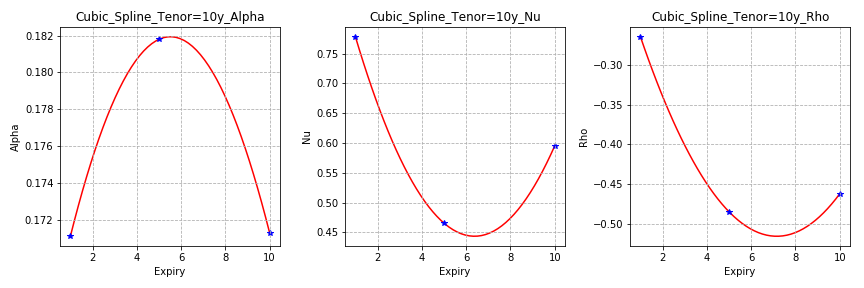
\includegraphics[scale=0.5]{Cubic_10y.png}
	\caption{Interpolation of SABR parameters - CMS10Y}
\end{figure}	

\noindent After interpolating all the SABR parameters, static replication is used to price each CMS rate and PV is the sum of the discounted values of all CMS rates, multiplied by the day count fraction. Here goes the mathematical form:
\begin{align*}
PV_{CMS10y}&=D(0,6m)\times 0.5 \times E^T [S_{6m,10y6m}(6m)] \\&+ D(0,1y) \times 0.5 \times E^T [S_{1y,11y}(1y)]\\&+ \dots 
+D(0,5y) \times 0.5 \times E^T [S_{5y,15y}(5y)]\\&= 0.213606
\end{align*}



\noindent Similarly, for CMS2y processed quarterly, $\alpha$ $\nu$, and $\rho$ can be interpolated between $1y$ $\times$ $2y$, $5y\times2y$,$10y\times2y$, whose profiles are demonstrated below:

\begin{figure}[h]
	\centering
	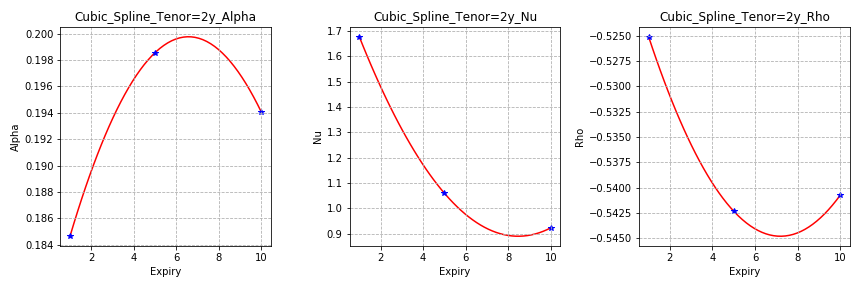
\includegraphics[scale=0.5]{Cubic_2y.png}
	\caption{Interpolation of SABR parameters - CMS2Y}
\end{figure}	

\noindent In addition to SABR parameters interpolation, due to quarterly arrangement, more discrete OIS discount rates and Libor discount rates are interpolated based on DF calculated in Section 1. After getting all the inputs, we can calculate PV of CMS2y as follow:
\begin{align*}
PV_{CMS2y}&=D(0,3m)\times 0.25 \times E^T [S_{3m,2y3m}(3m)] \\&+ D(0,6m) \times 0.25 \times E^T [S_{6m,2y6m}(6m)]\\&+ \dots 
+D(0,10y) \times 0.25 \times E^T [S_{10y,12y}(10y)]\\&= 0.504841
\end{align*}

\newpage

\noindent \textbf{CMS VS Par Swap Rate}\\ \\
Through trial and error, we found out that the CMS rates can become unlikely large numbers or even drop below par swap rate when upper bound for payer swaption integral is set as a large number or infinity. To figure out the optimal upper bound that not only covers most of the cases but generates plausible CMS rates, we calculated pure $f(K)$ in CMS rate formula by setting the payoff function as constant 1. When the upper bound is 0.85, no value exceeded 1, and CMS rates converged on reasonable readings.

\begin{figure}[h]
	\centering
	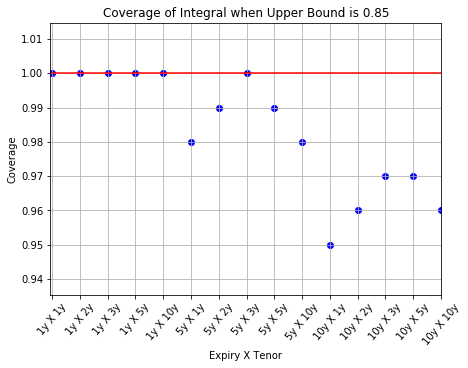
\includegraphics[scale=0.48]{Coverage.png}
	\caption{Coverage of Integral inside of CMS rate when Upper Bound is 0.85}
\end{figure}

Tables presented below show CMS rates for each maturity and tenor. 

\begin{figure}[h]
	\centering
	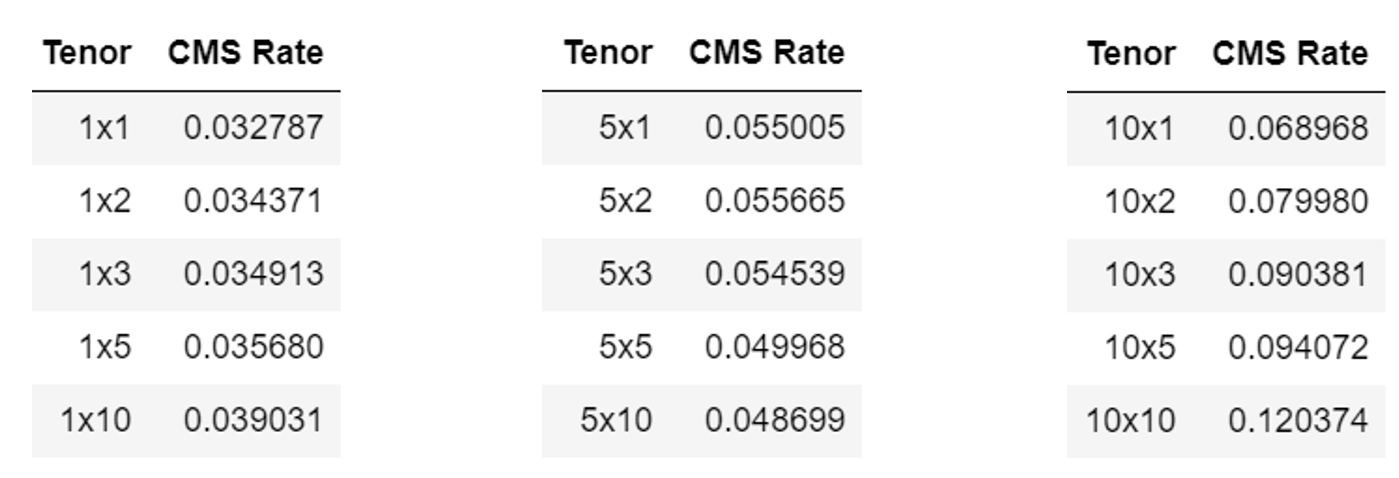
\includegraphics[scale=0.40]{CMS_RATE.png}
	\caption{CMS rates}
\end{figure}

\noindent Comparing CMS rates with forward swap rates of corresponding expiry and tenor which are derived from Part 1, we can recognise that the difference between CMS and forward swap rate increases as the expiry lengthens. It means that the longer expiry becomes, the greater the magnitude of convexity correction grows. On the contrary, the influence of tenor on the convexity correction is irregular. This phenomenon is presumed to be a result of volatility smile. 

\begin{figure}[ht]
	\centering
	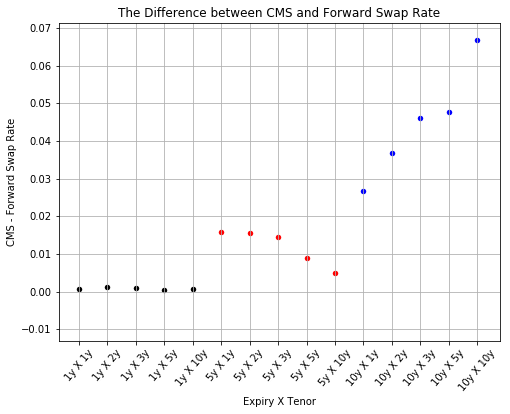
\includegraphics[scale=0.45]{CMS_FSR.png}
	\caption{Delta Profile for Up-and-In Barrier Option of Given Condition}
\end{figure}

\newpage

\par \noindent \textbf{Part IV - Decompounded Options}\\
\par \noindent \textbf{Question 1}\\

\noindent Starting from the generic contract valuation formula, we were able to obtain the static replication formula for the contract in question by first applying Leibniz's Rule on the IRR Payer and Receiver swaption formulas twice, after which integration by parts was carried out twice on the integrals in the generic contract valuation formula. \\

\noindent First, applying Leibniz's rule on the IRR Payer and Receiver swaption formulas twice yields:\\ \\
\noindent
\begin{minipage}[c]{0.5\textwidth}
	\begin{tcolorbox}[height=3.5cm,boxsep=5pt,arc=0pt,auto outer arc,colback=white,colframe=black]
		\noindent \textbf{Payer IRR Swaption}
		$$V^{pay}(K) = D(0,T) \int_{K}^{\infty} IRR(S) \cdot (S-K) \cdot f(S) dS$$
		$$\frac{\partial^2 V^{pay} (K)}{\partial K^2} = D(0,T) \cdot IRR(K) \cdot f(K)$$
	\end{tcolorbox}
\end{minipage}
\begin{minipage}[c]{0.5\textwidth}
	\begin{tcolorbox}[height=3.5cm,boxsep=5pt,arc=0pt,auto outer arc,colback=white,colframe=black]
		\noindent \textbf{Receiver IRR Swaption}
		$$V^{rec}(K) = D(0,T) \int_{0}^{F} IRR(S) \cdot (K-S) \cdot f(S) dS$$
		$$\frac{\partial^2 V^{rec} (K)}{\partial K^2} = D(0,T) \cdot IRR(K) \cdot f(K)$$
	\end{tcolorbox}
\end{minipage}\\ \\

\noindent We are now able to denote the generic contract valuation formula as such:
\begin{flalign*}
V_0 &= D(0,T)\mathbb{E} \left[ g(S) \right]\\
&=D(0,T) \int_{0}^{\infty} g(K) f(K) dK\\
&= \int_{0}^{F} h(K) \frac{\partial^2 V^{rec} (K)}{\partial K^2} dK + \int_{F}^{\infty} h(K) \frac{\partial^2 V^{pay} (K)}{\partial K^2} dK
\end{flalign*}\\

\noindent Integration by parts twice yields:
$$ V_0=D(0,T)g(F) + \int_{0}^{F} h''(K) V^{rec}(K)dK + \int_{F}^{\infty} h''(K) V^{pay}(K)dK $$

\noindent Where:\\
$$ F=S_{n,N}(0), \quad n=5, \quad N=15, \quad T=5 $$

$$ g(K) = K^{\frac{1}{p}} - 0.04^{\frac{1}{q}} = K^{\frac{1}{4}}-0.2, \quad
g'(K) = \frac{1}{4} K^{-\frac{3}{4}}, \quad
g''(K) = -\frac{3}{16}K^{-\frac{7}{4}} $$

$$ h(K) = \frac{g(K)}{IRR(K)}, \quad
h'(K) = \frac{IRR(K)g'(K)-g(K)IRR'(K)}{IRR(K)^2} $$

$$ h''(K) = \frac{IRR(K)g''(K)-IRR''(K)g(K)-2IRR'(k)g'(K)}{IRR(K)^2} + \frac{2IRR'(K)^2g(K)}{IRR(K)^3} $$

$$ V^{rec}=D(0,T) \cdot IRR(S_{n,N}(0)) \cdot \textnormal{Black76Put}(S_{n,N}(0),K,\sigma_{\textnormal{SABR}},T) $$

$$ V^{pay}=D(0,T) \cdot IRR(S_{n,N}(0)) \cdot \textnormal{Black76Call}(S_{n,N}(0),K,\sigma_{\textnormal{SABR}},T) $$\\

\noindent Using these parameters, we were able to obtain a Present Value (PV) for the $V_0$ of \textbf{0.2334}. $V_0$ can also be seen as a forward contract on the 10-year CMS rate with forward price set at 0.0016.

\newpage

\par \noindent \textbf{Question 2}\\

\noindent The contract ($V_0^+$) can be valued as though it is a CMS caplet when the payoff is $(S_T^{1/4}-0.04^{1/2})^+$.\\ \\
\noindent For $S_T^{1/4}-0.04^{1/2}$ to be positive:
\begin{flalign*}
S_T^{1/4}& >0.2\\
S_T &> 0.0016 = L
\end{flalign*}

\noindent Thus, we can see $V_0^+$ as a CMS caplet struck at $L=0.0016$:

\begin{flalign*}
V_0^+ &= D(0,T) \int_{L}^{\infty} g(K)f(K) dK\\
&=\int_{L}^{\infty} h(K) \frac{\partial^2 V^{pay }(K)}{\partial K^2} dK\\
&= h'(L) V^{pay} (L) + \int_{L}^{\infty} h''(K) V^{pay}(K)dK
\end{flalign*}

\noindent Using this valuation formula and relevant parameters from Question 1, we were able to obtain a Present Value (PV) for $\boldsymbol{V_0^+}$\textbf{ of 0.2430}, which is higher than $\boldsymbol{V_0}$\textbf{'s value of 0.2334}. \\ \\

\noindent This is intuitive as $V_0^+$ omits the negatively valued region of $V_0$ where $S_T < L$ and as such should be valued higher than $V_0$. It also follows that $V_0<V_0^+< \mathbb{E} \left[S_T^{1/4}\right]$ (spot price of the underlying), as this is the model-free no-arbitrage boundary that the three products must satisfy. Running further diagnostics, it can be seen that $V_0^+$ is consistently more highly priced than $V_0$ across the given values of $N$ (swap end date) for every $n$ (swap start date):

\begin{figure}[h]
	\centering
	\subcaptionbox{\label{}}{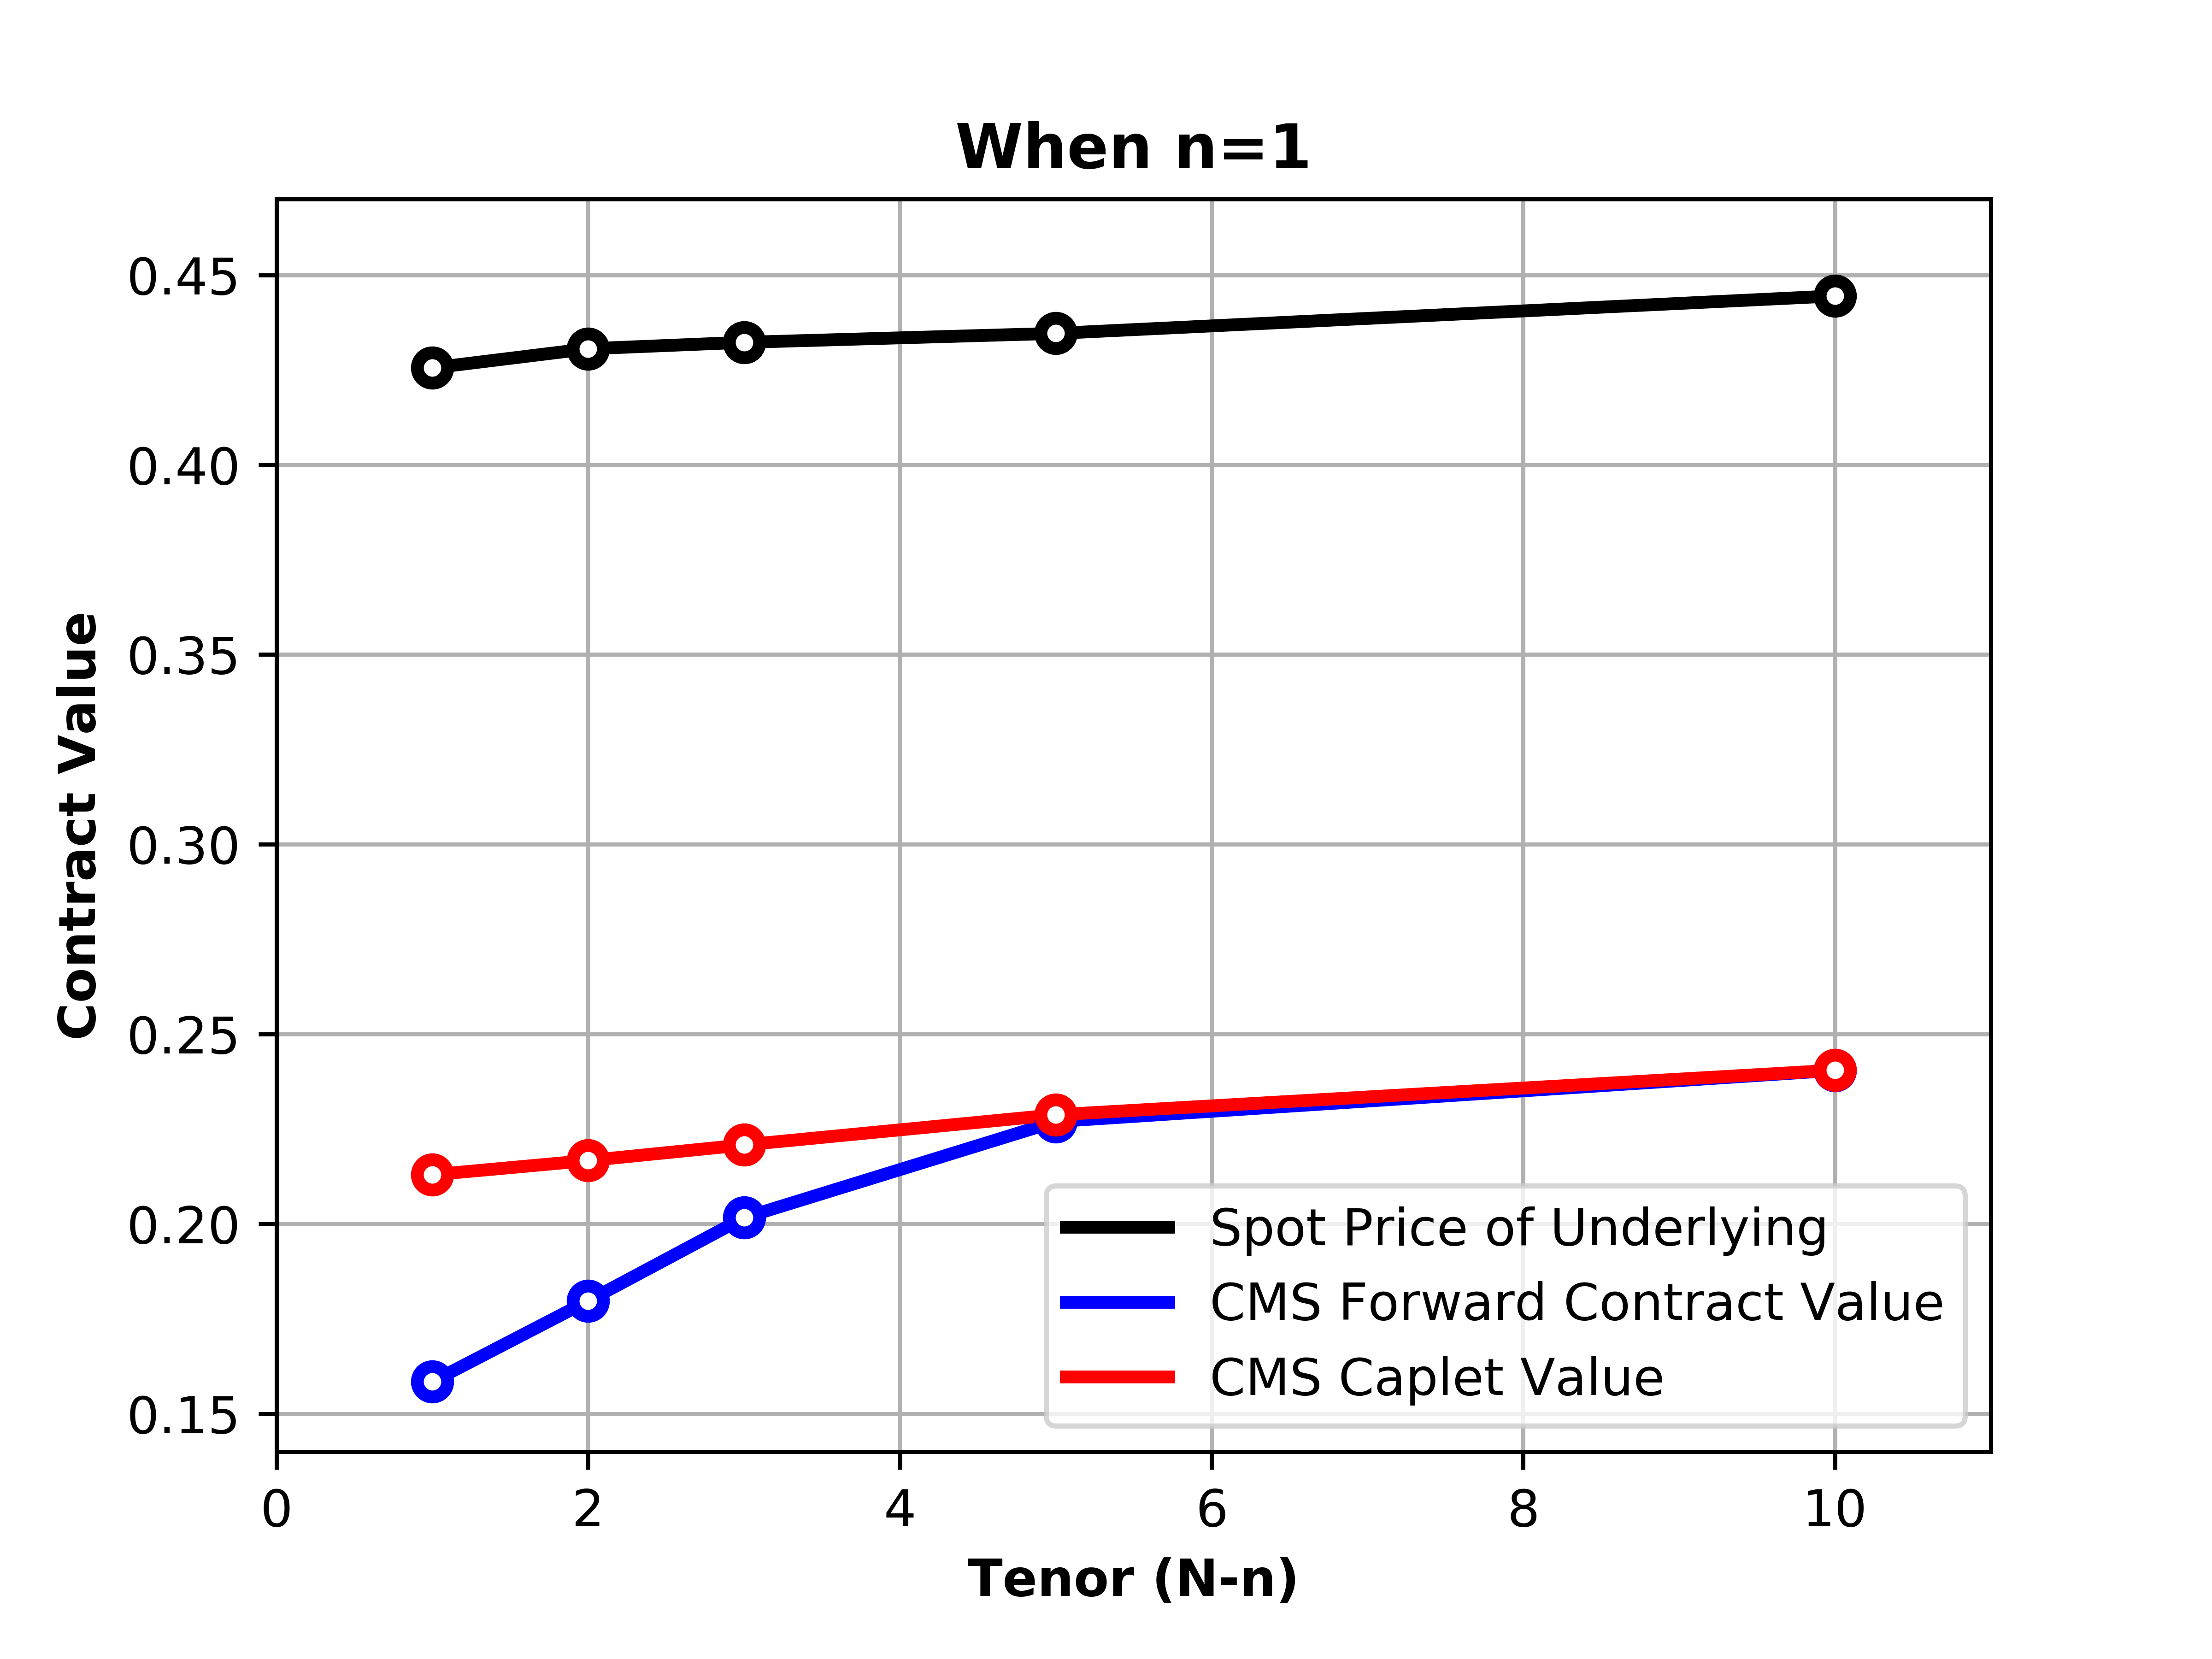
\includegraphics[width=.48\linewidth]{./P4n1.png}}\hspace{0.05em}
	\subcaptionbox{\label{}}{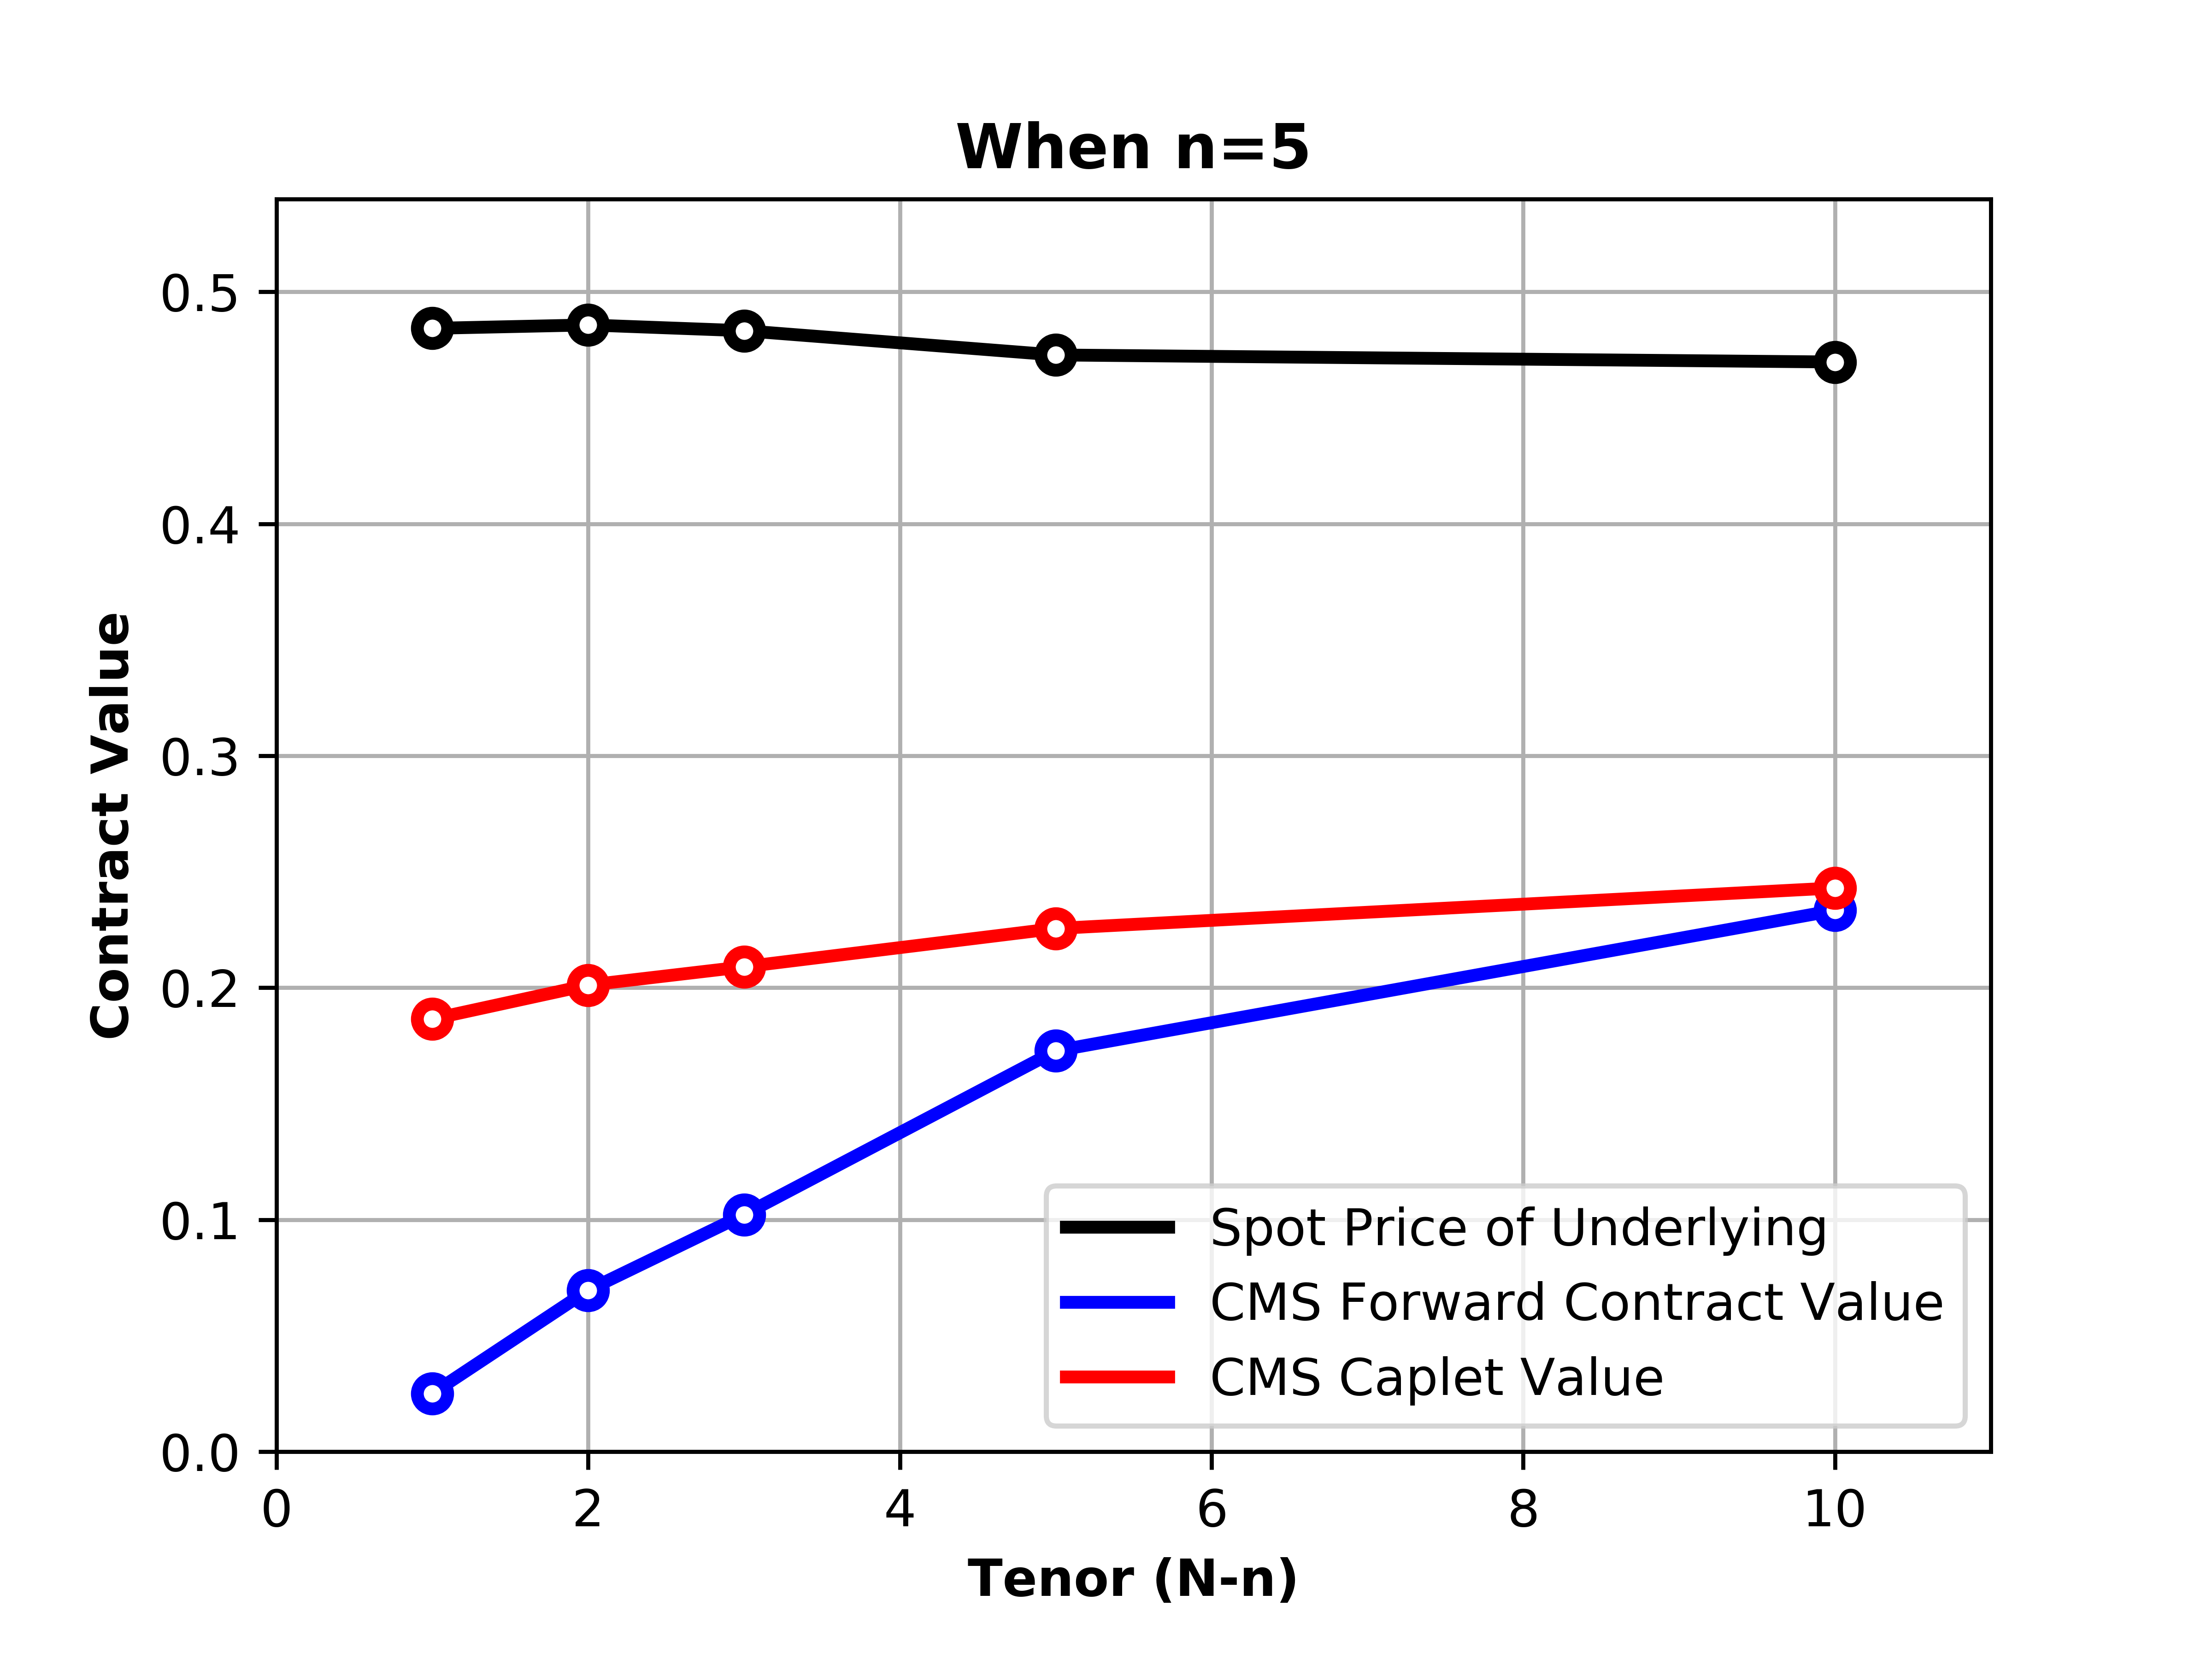
\includegraphics[width=.48\linewidth]{./P4n5.png}}\hspace{0.05em}
	\subcaptionbox{\label{}}{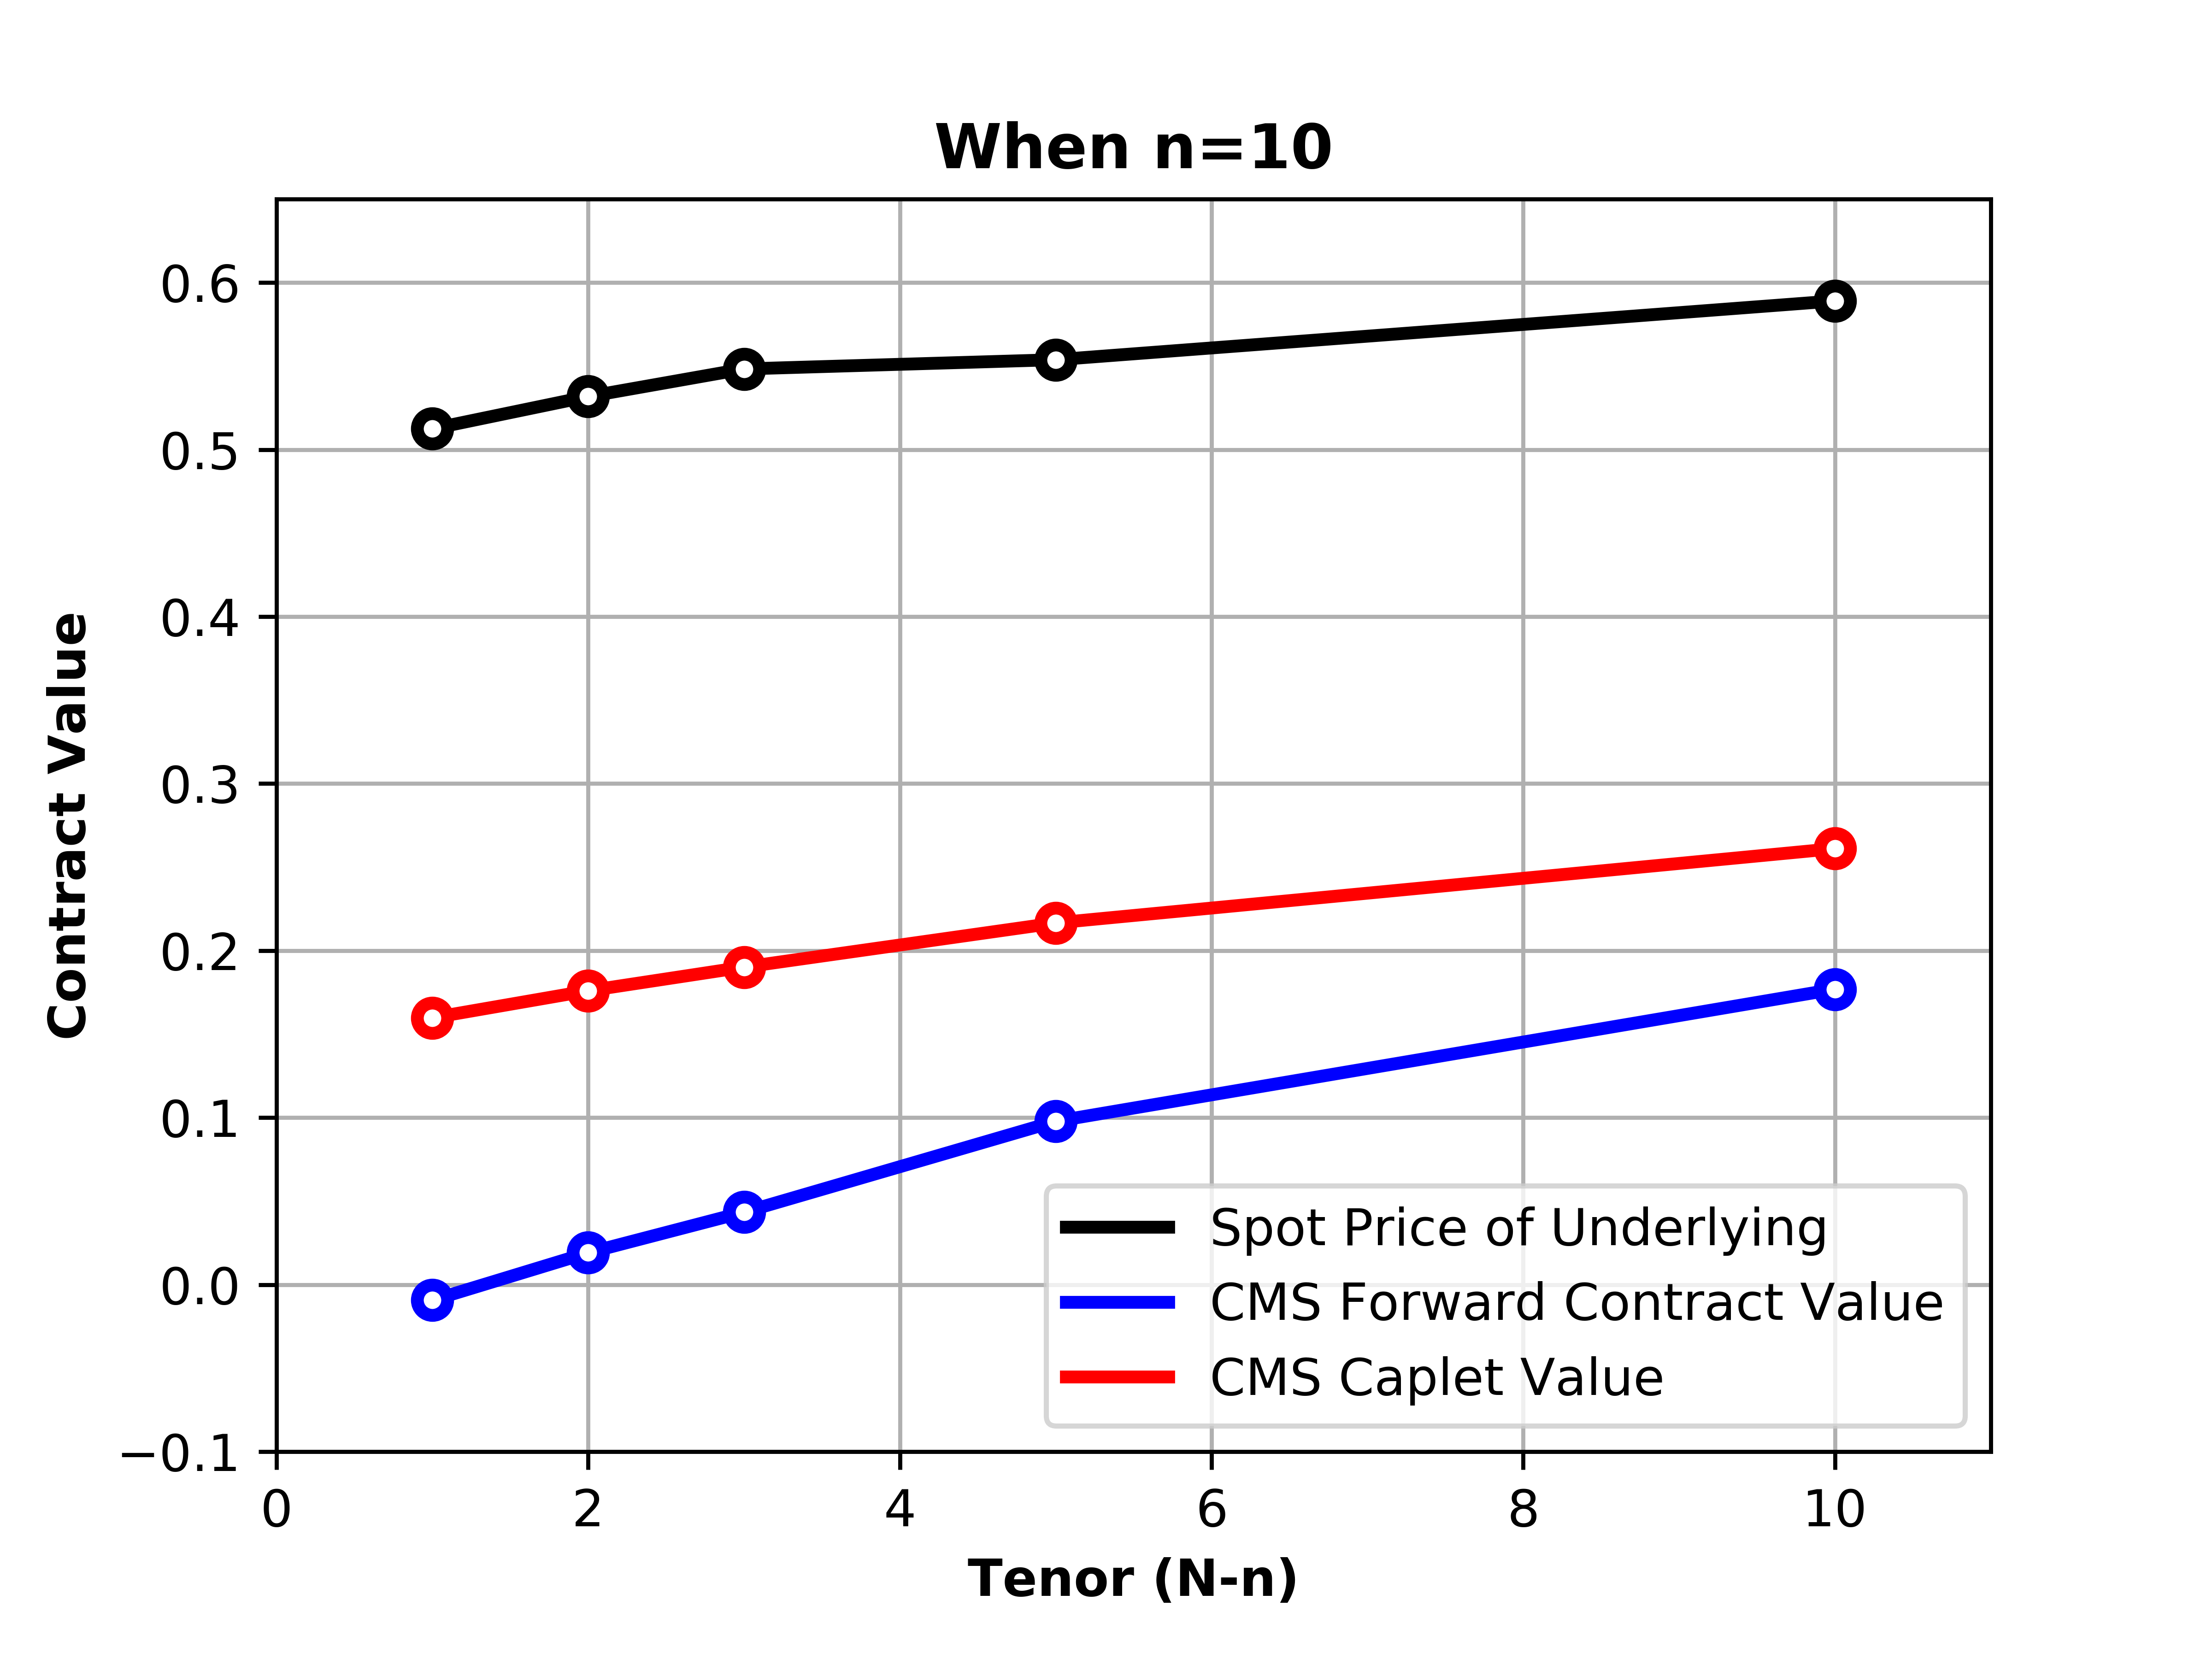
\includegraphics[width=.48\linewidth]{./P4n10.png}}
\end{figure}


\end{document}